\chapter{面向天基协同计算的区块链平台架构与运行机制}
\label{chap:platform}

前文已经围绕天基网络协同计算卸载问题分别完成了系统建模、系统层协同优化与任务层实时决策方法设计。第2章建立了面向天基协同计算的系统模型，刻画了节点异构、链路时变、任务随机到达与多主体协作等基本特征；第3章提出了基于区块链与多智能体强化学习的系统层协同资源分配方法，从全局尺度解决去中心化环境下的可信状态共享、信誉约束与多节点协同博弈问题；第4章进一步提出了基于联邦学习与深度强化学习的并发感知任务卸载方法，从任务到达瞬间的局部尺度解决链上状态滞后、节点数据隐私受限和多任务并发扰动条件下的实时决策问题。至此，本文已经形成了“系统层可信协同—任务层实时执行”的双层智能优化框架。

然而，模型与算法本身并不自动等价于可持续运行的分布式系统。系统层协同优化需要可信的状态同步、规则约束、信誉演化和行为审计作为支撑；任务层实时卸载需要候选节点摘要查询、联邦模型版本治理、任务生命周期记录和执行结果回流作为支撑。如果缺少统一的平台承载机制，第3章与第4章提出的方法将容易停留在离线仿真或局部模块验证层面，难以在真实天基分布式环境中形成稳定、可信、可追溯且可持续演化的运行闭环。因此，本章重点回答如下问题：如何设计一种面向天基协同计算的轻量级区块链平台，使系统层多智能体协同资源分配结果能够约束任务层卸载决策，并使任务层执行反馈能够反向更新系统层状态与信誉治理。

针对上述问题，本章提出一种面向双层智能协同计算的分层联盟链平台架构。该平台并非将区块链作为外置安全模块，而是将其作为连接系统层资源协同、任务层实时卸载、联邦模型治理与执行反馈审计的可信运行底座。平台通过主链—子链协同、链上/链下分离存储、智能合约治理与跨层状态接口，实现关键状态摘要共享、任务生命周期存证、模型版本溯源、信誉更新与异常隔离等功能。由此，第3章的系统层协同策略不再只是算法输出，而是可被平台记录、验证并转化为任务层可执行约束；第4章的任务层卸载行为也不再只是局部动作，而是能够通过链上事件回流为系统层状态更新和长期策略迭代提供依据。

本章后续内容安排如下。第\ref{sec:platform_requirement}节给出平台设计需求与问题定义，明确第五章与前文算法章节之间的边界；第\ref{sec:platform_architecture}节给出平台总体架构、网络映射与状态模型；第\ref{sec:hierarchical_chain}节设计分层联盟链、区块结构和链上/链下协同存证机制；第\ref{sec:contract_governance}节给出智能合约与可信治理机制；第\ref{sec:method_mapping}节重点说明系统层方法与任务层方法的平台映射及跨层运行闭环；第\ref{sec:platform_evaluation}节从确认时延、存储开销、异常隔离和方法承载关系等角度分析工程可行性；最后第\ref{sec:platform_summary}节对本章进行总结。

\section{平台设计需求与问题定义}
\label{sec:platform_requirement}

\subsection{平台设计动因}

天基协同计算卸载问题并不是单一任务的转发或调度问题，而是在动态网络条件下由多类异构节点共同参与的状态感知、资源竞争、任务迁移、模型更新、行为反馈与规则治理问题。卫星节点既可能作为任务发起方，也可能作为协同计算资源提供方；节点之间在共享算力、存储、链路与能量资源的同时，还受到拓扑时变、链路窗口受限、任务突发到达和节点能力异构等因素影响。仅依靠单节点局部决策或单次优化求解，难以从根本上解决天基环境中的持续协同问题。

第3章从系统层角度构建了区块链增强的多智能体协同资源分配方法，重点解决多节点在全局资源竞争背景下如何实现可信状态共享、信誉激励与协同策略学习。该方法成立的前提是系统中存在一个能够维护公共状态摘要、信誉记录和治理规则的可信环境。如果不同节点之间缺乏一致的状态同步与审计机制，系统层智能体获取的全局状态可能受到局部偏差、延迟上报甚至虚假上报影响，从而削弱系统层协同优化的有效性。

第4章从任务层角度提出了基于联邦学习与深度强化学习的并发感知卸载方法，重点解决新任务到达时节点如何结合本地观测、候选节点摘要和并发开销预测结果做出实时卸载决策。该方法依赖联邦预测模型的持续更新、模型参数的一致性校验、任务执行结果的回流反馈以及跨节点行为的可追溯记录。如果缺乏统一平台，任务层方法虽然能够在局部条件下形成卸载动作，但其模型版本治理、执行结果可验证性和长期策略迭代能力难以保证。

因此，本章的平台设计不是在前文之外额外增加一个孤立模块，而是面向“双层智能方法如何在分布式天基环境中运行”这一问题，建立统一的可信承载机制。其核心目标是将系统层的全局协同结果转化为任务层的可执行约束，并将任务层的执行结果反向沉淀为系统层的可信状态、信誉更新和策略迭代依据。

\subsection{章节边界与平台需求}

为了避免第五章与第3章、第4章在区块链功能描述上产生重复，有必要先明确三者的研究边界。第3章中的区块链主要服务于系统层协同资源分配算法，承担公共博弈信息板的角色；第4章中的区块链主要服务于任务层实时卸载算法，维护候选节点摘要、任务事件和模型版本凭据；本章则从平台层出发，关注这些链上能力如何被组织为统一、可运行、可扩展的系统架构，并进一步支撑双层智能方法之间的约束传递与反馈闭环。表\ref{tab:chapter_boundary}给出了三者之间的差异。

\begin{table}[htbp]
  \centering
  \caption{第3章、第4章与第5章的研究边界对比}
  \label{tab:chapter_boundary}
  \begin{tabular}{p{2.2cm}p{3.5cm}p{3.5cm}p{3.8cm}}
    \toprule
    对比维度 & 第3章 & 第4章 & 第5章 \\
    \midrule
    研究对象 & 系统层协同资源分配 & 任务层并发感知卸载 & 双层智能方法的平台化承载 \\
    区块链角色 & 公共博弈信息板 & 可信但非实时的状态与模型凭据 & 可信运行底座与治理框架 \\
    核心数据 & 负载摘要、信誉状态、策略行为 & 候选节点摘要、任务事件、模型版本 & 任务生命周期、模型治理、跨链摘要、审计索引 \\
    主要输出 & 资源协同动作与信誉激励 & 本地执行或目标节点卸载动作 & 约束传递、存证审计、反馈回流与工程承载 \\
    验证重点 & 收敛性、负载均衡、抗自私行为 & 时延、能耗、并发开销、鲁棒性 & 共识开销、存储增长、异常治理、可部署性 \\
    \bottomrule
  \end{tabular}
\end{table}

基于上述边界，平台设计需要满足以下需求。

第一，可信状态共享需求。平台需要对节点资源状态、链路统计、任务分布、信誉评分和模型版本等关键信息进行摘要化维护，为系统层与任务层智能决策提供一致、可验证且可追溯的公共状态视图。考虑到天基网络链路带宽有限和可见窗口受限，平台不宜将高维原始数据全部上链，而应采用摘要上链与实体链下存储相结合的方式。

第二，跨层约束传递需求。系统层方法输出的资源边界、节点可调度集合、服务能力约束和信誉状态，需要被平台转化为任务层可读取的约束条件，使任务层卸载决策不再仅依赖瞬时局部观测，而是在系统层全局协同结果约束下完成动作选择。

第三，任务生命周期治理需求。任务从生成、提交、接纳、执行、完成到失败回退的全过程都应形成可追溯事件链。平台需要记录任务关键状态迁移、目标节点选择、执行结果摘要和异常事件，以支撑后续审计、信誉更新和策略改进。

第四，模型版本可信治理需求。第4章中的联邦预测模型和任务层DQN策略模型都具有持续演化特征。平台需要维护模型版本号、参数哈希、聚合轮次、适用簇编号和性能摘要等信息，保证节点在调用模型前能够验证模型来源和版本合法性。

第五，轻量化与可部署需求。天基节点算力、能量和通信资源受限，平台不能采用高消耗共识或全量数据上链机制。平台设计应控制共识节点规模、降低交易确认时延、压缩链上数据规模，并通过主链—子链结构提高局部业务处理效率。

\section{平台总体架构与状态模型}
\label{sec:platform_architecture}

\subsection{平台总体架构}

为支撑天基协同计算环境下“资源状态可信同步—系统层协同决策—任务层动态卸载—执行结果审计反馈”的完整闭环，本章设计一种面向动态星地网络的区块链协同计算平台总体架构，如图\ref{fig:platform-arch}所示。平台整体划分为基础设施与网络环境层、区块链平台核心层、双层智能决策层以及应用与管理层四个层次。

基础设施与网络环境层由卫星终端、卫星边缘节点、地面站、边缘计算集群、地面云以及星间/星地链路构成，负责提供计算、存储、通信和能量等物理资源。该层产生的原始状态包括节点CPU利用率、队列长度、缓存占用、剩余能量、链路速率、传播时延、可见窗口和任务到达过程等，是后续链上摘要和智能决策的基础来源。

区块链平台核心层是平台实现可信协同的中枢，主要包括身份认证、轻量级共识、分层账本、跨链网关、链上/链下存储、智能合约、状态摘要维护和审计查询等模块。该层不直接替代实时调度器，而是通过维护可信摘要、规则状态、任务事件和模型版本，为系统层和任务层决策提供统一的可信上下文。

双层智能决策层对应第3章和第4章提出的两类方法。系统层协同资源分配模块面向较长时间尺度，根据链上公共状态、节点信誉和任务统计信息输出资源协同策略、节点调度边界和服务能力约束；任务层并发感知卸载模块面向较短时间尺度，在单个任务到达时读取本地状态、候选节点摘要、系统层约束和联邦预测结果，输出本地执行或目标节点卸载动作。

应用与管理层面向应急遥感、星座协同处理、空间态势感知、区域目标识别、任务监管和可视化运维等场景，提供任务发布、服务部署、模型管理、日志分析、异常告警和审计查询等能力。该层使平台不仅能够服务于算法验证，也能够形成面向工程部署的可观测、可配置和可审计环境。

\begin{figure}[htbp]
  \centering
  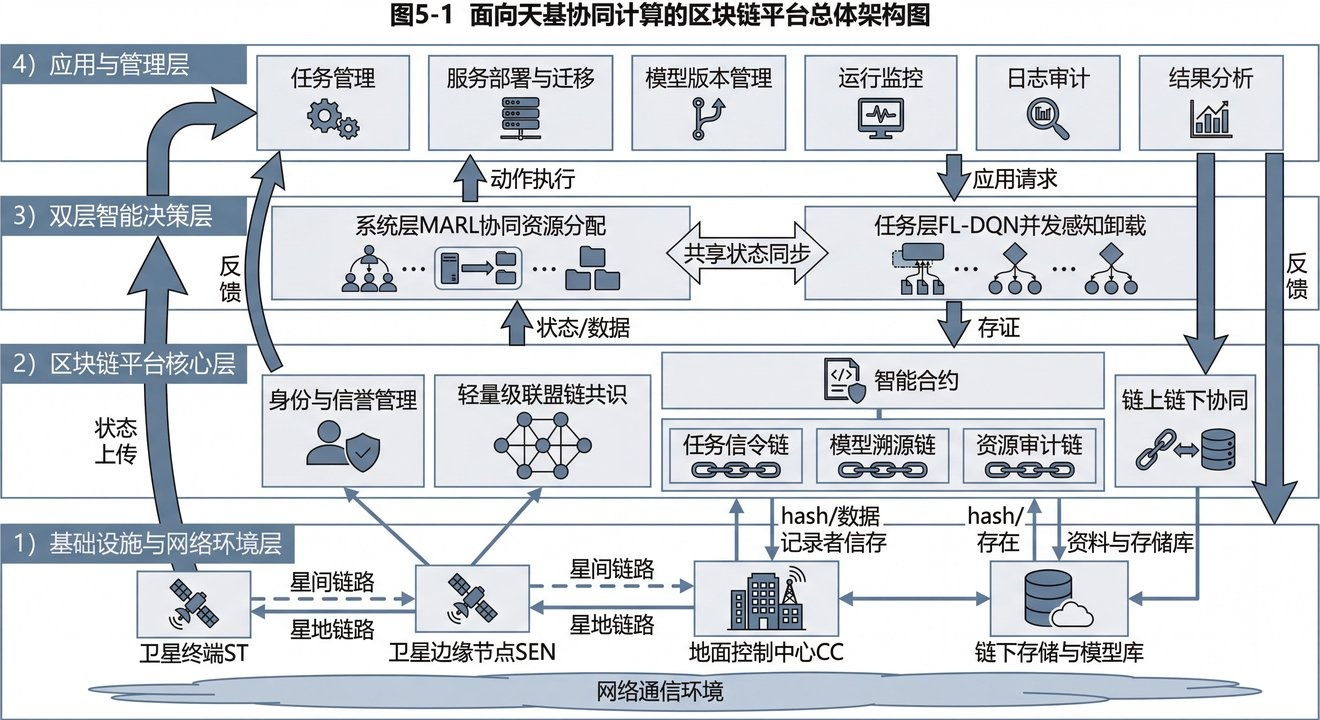
\includegraphics[width=0.96\textwidth]{figures/5-1.jpeg}
  \caption{面向天基协同计算的区块链平台总体架构图}
  \label{fig:platform-arch}
\end{figure}

上述四层结构的关键不在于简单分层，而在于形成了“状态感知—链上同步—联合决策—执行反馈”的运行闭环。基础设施层产生的动态状态首先经过摘要化处理进入区块链核心层；系统层和任务层智能模块再基于链上可信摘要与本地观测进行决策；决策结果以任务事件、策略摘要和执行反馈形式写回链上；链上状态进一步影响后续资源协同、模型更新与信誉演化。

\subsection{网络映射与节点角色}

平台将天基协同网络抽象为时变有向图
\begin{equation}
  \mathcal{G}(t)=\big(\mathcal{V},\mathcal{E}(t)\big),
  \label{eq:platform_graph}
\end{equation}
其中，\(\mathcal{V}\)表示参与天基协同计算与区块链维护的星地节点集合，\(\mathcal{E}(t)\)表示随轨道运动、可见窗口和链路拥塞状态动态变化的星间或星地通信连接集合。进一步地，平台将节点划分为共识维护节点集合\(\mathcal{C}\)、业务执行节点集合\(\mathcal{L}\)和链下存储/服务节点集合\(\mathcal{D}\)，满足
\begin{equation}
  \mathcal{C}\subseteq \mathcal{V}, \qquad \mathcal{L}\subseteq \mathcal{V}, \qquad \mathcal{D}\subseteq \mathcal{V}.
  \label{eq:node_sets}
\end{equation}

共识维护节点负责区块打包、交易验证、状态定序和全局摘要广播，可由具备较高稳定性、较强计算能力和较好通信条件的卫星边缘节点或地面控制节点承担。业务执行节点负责发起任务、接收任务、执行卸载动作、采集状态和上报结果。链下存储/服务节点负责保存原始任务数据、完整模型参数、服务镜像和大规模运行日志，并通过哈希索引与链上摘要建立可验证映射。

为了将任务调度对象纳入平台治理框架，本章进一步将平台中的任务—资源映射表示为
\begin{equation}
  \mathrm{SNEMS}=\{T,R,X,F\},
  \label{eq:snems}
\end{equation}
其中，\(T\)表示待调度任务集合，\(R\)表示由平台集、载荷集、窗口集和执行时机构成的资源集合，\(X\)表示任务—资源决策矩阵，\(F\)表示由硬约束和收益函数构成的评价集合。该表示并不替代第2章的系统模型，而是为平台层补充统一接口：任务如何进入链上治理，资源如何进入系统层动作空间，局部卸载动作如何受全局约束影响，以及执行结果如何回流为新的评价依据。

\subsection{平台状态模型}

为支撑后续智能合约、跨层接口和反馈闭环设计，平台需要形成统一的状态表示。设平台在时刻\(t\)的状态为
\begin{equation}
  S_p(t)=\big\{S_{\mathrm{res}}(t),S_{\mathrm{task}}(t),S_{\mathrm{model}}(t),S_{\mathrm{rep}}(t),S_{\mathrm{audit}}(t)\big\},
  \label{eq:platform_state}
\end{equation}
其中，\(S_{\mathrm{res}}(t)\)表示资源状态，包括节点负载、可用算力、存储占用、剩余能量和链路统计；\(S_{\mathrm{task}}(t)\)表示任务状态，包括任务提交、接纳、执行、完成、失败和回退等生命周期事件；\(S_{\mathrm{model}}(t)\)表示模型状态，包括联邦预测模型、DQN策略模型和系统层策略模型的版本号、哈希摘要、适用范围和性能摘要；\(S_{\mathrm{rep}}(t)\)表示信誉状态，包括节点历史服务质量、异常记录、任务完成率和信誉评分；\(S_{\mathrm{audit}}(t)\)表示审计状态，包括合约调用日志、异常证据、访问记录和跨链锚定索引。

当新区块\(B_h\)通过共识确认后，平台状态按照合约规则集合完成更新：
\begin{equation}
  S_p(t+1)=\Gamma\big(S_p(t),B_h,\Omega_{\mathrm{contract}}\big),
  \label{eq:platform_state_update}
\end{equation}
其中，\(\Gamma(\cdot)\)表示状态转移函数，\(\Omega_{\mathrm{contract}}\)表示智能合约规则集合，具体包括节点准入规则、状态摘要规则、任务生命周期规则、模型版本规则、信誉更新规则和异常隔离规则。与传统数据库更新不同，式\eqref{eq:platform_state_update}中的状态转移具有可验证、可追溯和不可随意篡改的特征，为双层智能方法提供可信运行语义。

\section{分层联盟链与链上/链下协同机制}
\label{sec:hierarchical_chain}

\subsection{主链—子链结构设计}

天基协同计算平台中的业务事件在频率、时效性和安全等级方面存在明显差异。例如，节点身份、信誉锚定、治理规则和跨域审计具有全局性与稳定性，适合由主链维护；任务开始/结束事件、局部资源状态和业务日志更新频率较高，适合由子链快速记录；原始遥感数据、完整模型参数和详细执行日志体量较大，适合链下存储。因此，本章采用主链、子链和链下设备层协同的分层联盟链结构，如图\ref{fig:chain-arch}所示。

\begin{figure}[htbp]
  \centering
  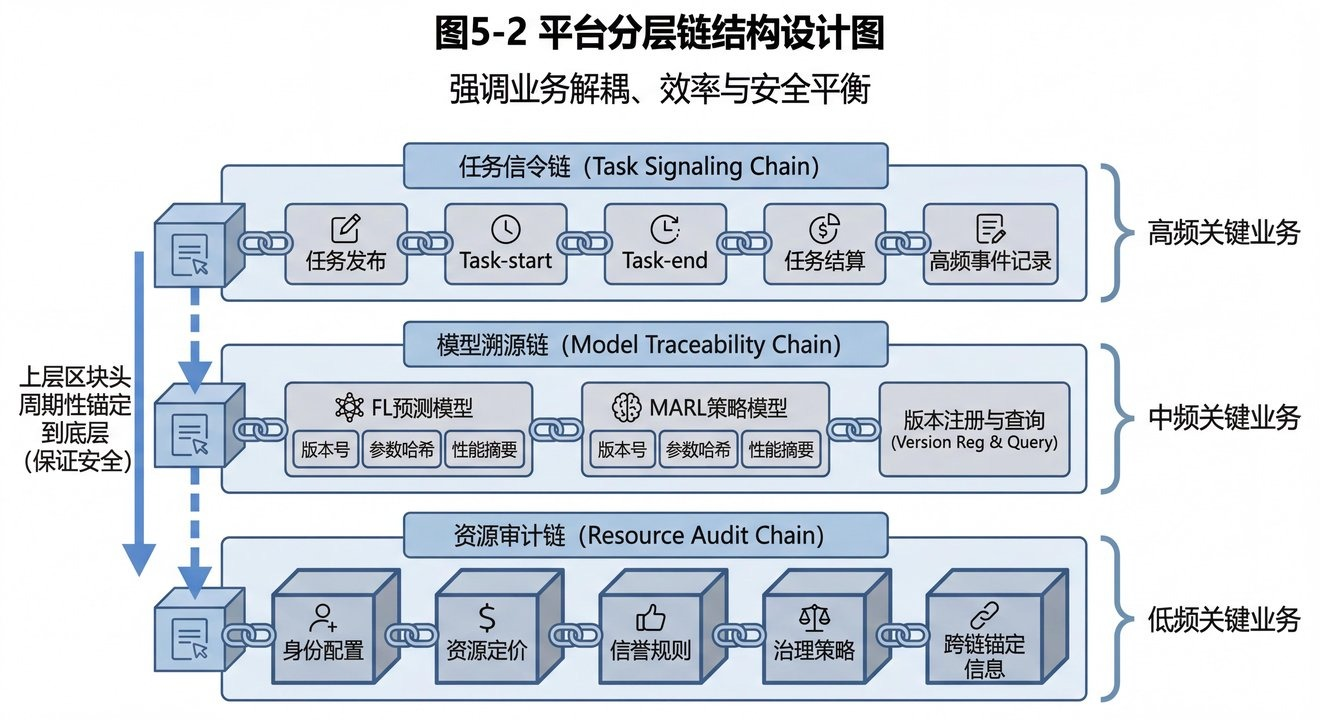
\includegraphics[width=0.92\textwidth]{figures/5-2.jpeg}
  \caption{平台分层链结构设计图}
  \label{fig:chain-arch}
\end{figure}

主链负责维护全局治理状态，主要包括节点身份、角色权限、信誉状态、治理规则、跨子链摘要、模型版本锚定和全局审计索引。主链更新频率相对较低，但其状态具有更强的系统级约束作用，是平台实现跨域一致性和长期治理的核心。

子链负责维护局部业务状态，可按照轨道区域、任务类型、星座分组或应用域划分。子链主要记录任务生命周期事件、局部资源摘要、局部行为审计记录和业务域内模型调用事件。相较于主链，子链更新周期更短，更适合承载快时标任务事件和局部调度信息。

链下设备层负责存储大规模实体对象，包括原始任务输入、遥感数据片段、完整模型参数、训练样本索引、服务镜像和详细日志。链下对象不直接进入账本，而是通过哈希指针、对象地址和访问权限记录与链上摘要建立映射关系。节点读取链下对象时，可通过链上哈希验证其完整性和一致性。

\subsection{区块结构设计}

为增强平台结构设计的可操作性，本章分别给出子链区块和主链锚定区块的字段化表达。设第\(s\)条子链在高度\(h\)处生成的区块为\(B_s^h\)，其结构可表示为
\begin{equation}
  B_s^h=\{h_s,t_s,ID_s,Root_{\mathrm{task}},Root_{\mathrm{state}},Root_{\mathrm{model}},Root_{\mathrm{audit}},H(B_s^{h-1}),Sig_{\mathcal{C}_s}\},
  \label{eq:sub_block}
\end{equation}
其中，\(h_s\)表示子链区块高度，\(t_s\)表示区块时间戳，\(ID_s\)表示子链标识，\(Root_{\mathrm{task}}\)表示任务生命周期事件根，\(Root_{\mathrm{state}}\)表示局部资源状态摘要根，\(Root_{\mathrm{model}}\)表示模型调用或版本摘要根，\(Root_{\mathrm{audit}}\)表示局部审计事件根，\(H(B_s^{h-1})\)表示前一区块哈希，\(Sig_{\mathcal{C}_s}\)表示子链共识节点签名集合。

主链在接收跨链网关提交的子链摘要后生成锚定区块。设主链在高度\(k\)处生成的区块为\(B_m^k\)，其结构可表示为
\begin{equation}
  B_m^k=\{h_m,t_m,Root_{\mathrm{subchain}},Root_{\mathrm{rep}},Root_{\mathrm{rule}},Root_{\mathrm{model}},Root_{\mathrm{global\_audit}},H(B_m^{k-1}),Sig_{\mathcal{C}_m}\},
  \label{eq:main_block}
\end{equation}
其中，\(Root_{\mathrm{subchain}}\)表示多个子链摘要的聚合根，\(Root_{\mathrm{rep}}\)表示节点信誉状态根，\(Root_{\mathrm{rule}}\)表示治理规则版本根，\(Root_{\mathrm{model}}\)表示全局模型版本锚定根，\(Root_{\mathrm{global\_audit}}\)表示跨子链审计索引根，\(Sig_{\mathcal{C}_m}\)表示主链共识节点签名集合。

上述设计相较于简单记录\(\{D_{\mathrm{hash}},H(B^-),H(B)\}\)的哈希链结构，能够更清晰地区分任务、状态、模型与审计信息的链上职责。子链通过高频记录局部任务与资源摘要保证快时标事件可追溯，主链通过低频锚定关键摘要保证全局规则、信誉和模型版本的一致性。

\subsection{链上/链下协同存证流程}

考虑到天基网络链路资源有限且任务数据体量较大，平台采用“链上保存摘要、链下保存实体对象”的分层存证方式。链上主要保存任务标识、状态摘要、模型版本哈希、审计索引、合约结果和关键治理规则等小体积但高价值信息；链下保存任务原始输入、完整模型参数、服务镜像、训练样本索引和详细日志等大规模对象。

设某一链下对象为\(D_j\)，其对象地址为\(Loc(D_j)\)，哈希摘要为
\begin{equation}
  digest_j=H(D_j\,\|\,Loc(D_j)\,\|\,t_j),
  \label{eq:data_digest}
\end{equation}
其中，\(H(\cdot)\)表示密码学哈希函数，\(t_j\)表示对象生成时间。平台仅将\(digest_j\)、对象类型、访问权限和索引信息写入链上。当节点需要读取链下对象时，先通过合约验证访问权限，再从链下存储获取对象并重新计算哈希；若计算结果与链上摘要一致，则认为对象未被篡改。

数据写入流程包括四个步骤。第一，业务节点生成任务输入、模型参数或执行日志等对象，并在本地或边缘存储节点完成链下保存。第二，业务节点计算对象哈希并向所属子链提交存证交易。第三，子链共识节点验证交易格式、权限和摘要合法性，确认后写入子链区块。第四，跨链网关周期性聚合子链摘要，并将其提交至主链完成全局锚定。

数据读取流程同样包括四个步骤。第一，请求节点向主链或子链提交读取请求，合约验证其身份和访问权限。第二，平台根据链上索引返回对象地址和哈希摘要。第三，请求节点从链下存储获取实体对象，并重新计算哈希。第四，若本地计算哈希与链上摘要一致，则允许进入后续模型推理、任务审计或结果复核流程；否则触发异常审计合约。

该机制能够在不显著增加链上存储压力的前提下，为任务数据、模型参数和执行日志提供完整性验证能力，适合天基网络中带宽受限、数据体量大且可信要求高的应用场景。

\section{智能合约与可信治理机制}
\label{sec:contract_governance}

\subsection{智能合约类型}

在分布式天基协同计算环境中，仅依赖人工配置或静态规则难以保证长期运行过程中的一致性和可审计性。为将任务流转、状态维护、模型治理和异常处理转化为可自动执行的规则，本章在平台中设计六类核心智能合约，如表\ref{tab:contract_design}所示。

\begin{table}[htbp]
  \centering
  \caption{平台核心智能合约设计}
  \label{tab:contract_design}
  \begin{tabular}{p{2.5cm}p{3.4cm}p{3.5cm}p{3.5cm}}
    \toprule
    合约类型 & 输入 & 输出 & 作用 \\
    \midrule
    节点准入合约 & 节点身份、证书、资源能力、角色申请 & 节点角色、权限集合、准入状态 & 控制共识节点、业务节点和链下服务节点的加入与退出 \\
    状态摘要合约 & 资源状态、链路统计、队列长度、时间戳 & 可信状态摘要、状态版本号 & 为系统层MARL和任务层DQN提供公共状态输入 \\
    任务生命周期合约 & 任务提交、接纳、开始、完成、失败事件 & 任务状态迁移记录、审计索引 & 支撑任务全过程存证与执行结果追溯 \\
    模型版本合约 & 模型编号、簇编号、聚合轮次、参数哈希、性能摘要 & 可验证模型版本、合法性状态 & 支撑联邦预测模型与策略模型的版本治理 \\
    信誉更新合约 & 执行结果、任务重要度、异常记录、链路状态 & 节点信誉值、奖惩结果 & 支撑系统层信誉激励与异常约束 \\
    异常隔离合约 & 异常证据、审计结果、重复违规次数 & 限权、降权或隔离动作 & 约束虚假上报、拒绝服务和恶意模型更新等行为 \\
    \bottomrule
  \end{tabular}
\end{table}

节点准入合约负责维护平台参与者的身份和权限。由于天基协同计算平台属于许可制联盟链，只有通过身份验证和能力评估的节点才能参与账本维护、任务执行、模型聚合或链下存储。该合约可根据节点类型为其分配不同角色，避免普通业务节点直接参与全局治理或访问不具备权限的数据对象。

状态摘要合约负责将高频原始状态转化为低维可信摘要。对于节点负载、链路带宽、队列长度和剩余能量等高频状态，平台不要求全量上链，而是通过摘要化和时间戳机制记录关键统计量。系统层智能体可使用这些摘要估计全局负载与协同关系，任务层智能体可使用这些摘要筛选候选卸载节点。

任务生命周期合约负责记录任务从生成到结束的关键状态迁移。任务提交时，合约登记任务标识、任务类型、输入数据摘要和截止期；目标节点接纳任务后，合约记录接纳时间、目标节点和约束版本；任务执行结束后，合约记录完成状态、时延、能耗、结果摘要和异常信息。该合约是任务行为可追溯和执行结果可验证的基础。

模型版本合约负责维护联邦预测模型、任务层DQN策略模型和系统层协同策略模型的版本信息。对于第4章中的联邦预测模型，合约记录模型所属簇、聚合轮次、参数哈希和性能摘要；对于策略模型，合约记录策略版本、训练时间、适用场景和回滚索引。节点在调用模型前可通过该合约验证模型版本，避免使用过期或被篡改的参数。

信誉更新合约负责将任务执行结果和异常审计结果转化为节点信誉变化。信誉值不仅影响第3章系统层协同资源分配中的奖励和约束，也可影响第4章联邦学习中的聚合权重和任务层候选节点优先级。异常隔离合约则负责对虚假上报、频繁拒绝任务、恶意提交模型更新或长期低质量服务等行为进行降权、限权或隔离处理。

\subsection{信誉更新与异常隔离}

设节点\(i\)在时间窗\(\tau\)内的信誉值为\(R_i(\tau)\)，平台可根据历史信誉和当前任务执行结果进行更新：
\begin{equation}
  R_i(\tau)=\alpha R_i(\tau-1)+(1-\alpha)\sum_{k\in\mathcal{T}_i(\tau)} I(\mathrm{link}_k)\,\omega_k\,\varphi_i(k),
  \label{eq:rep_update}
\end{equation}
其中，\(\alpha\in(0,1)\)表示历史遗忘因子，\(\mathcal{T}_i(\tau)\)表示节点\(i\)在时间窗\(\tau\)内参与处理的任务集合，\(I(\mathrm{link}_k)\)表示任务执行期间相关链路是否处于可用状态，\(\omega_k\)表示任务重要度权重，\(\varphi_i(k)\)表示任务\(k\)的执行评价函数。评价函数可由任务完成状态、完成时延、能耗偏差、结果质量和异常标记共同构成：
\begin{equation}
  \varphi_i(k)=\lambda_1 q_k-\lambda_2 \frac{L_k}{D_k}-\lambda_3 \frac{E_k}{E_k^{\max}}-\lambda_4 \xi_k,
  \label{eq:exec_score}
\end{equation}
其中，\(q_k\)表示任务完成质量，\(L_k\)表示实际完成时延，\(D_k\)表示任务截止期，\(E_k\)表示实际能耗，\(E_k^{\max}\)表示可接受能耗上界，\(\xi_k\)表示异常惩罚项，\(\lambda_1,\lambda_2,\lambda_3,\lambda_4\)为权重系数。

当节点信誉低于阈值\(R_{\min}\)或在连续时间窗内出现异常行为时，异常隔离合约触发限权机制：
\begin{equation}
  \mathcal{P}_i(\tau+1)=\Psi\big(\mathcal{P}_i(\tau),R_i(\tau),N_i^{\mathrm{abn}}(\tau)\big),
  \label{eq:permission_update}
\end{equation}
其中，\(\mathcal{P}_i(\tau)\)表示节点权限集合，\(N_i^{\mathrm{abn}}(\tau)\)表示异常次数，\(\Psi(\cdot)\)表示权限更新函数。权限调整可以表现为降低候选节点优先级、削弱联邦聚合权重、暂停任务接纳资格或移出共识节点集合。

\section{双层智能方法的平台映射与运行闭环}
\label{sec:method_mapping}

\subsection{系统层协同资源分配方法的平台映射}

第3章提出的区块链增强多智能体协同资源分配方法，核心在于利用联盟链公共信息板提供可信公共摘要，并在多智能体强化学习框架下实现系统层资源协同。映射到本章平台后，该方法被部署在双层智能决策层的系统层控制模块中，其输入、输出和链上接口如表\ref{tab:ch3_mapping}所示。

\begin{table}[htbp]
  \centering
  \caption{系统层协同资源分配方法的平台映射}
  \label{tab:ch3_mapping}
  \begin{tabular}{p{2.8cm}p{4.2cm}p{4.0cm}p{3.0cm}}
    \toprule
    第3章要素 & 平台承载对象 & 链上记录内容 & 平台作用 \\
    \midrule
    公共状态摘要 & 状态摘要合约与公共信息板 & 全局负载、负载方差、链路统计、任务分布 & 为MARL提供可信状态输入 \\
    信誉激励 & 信誉更新合约 & 节点信誉值、奖惩记录、异常索引 & 约束自利行为并影响后续调度 \\
    系统层动作 & 资源协同策略接口 & 资源边界、候选节点优先级、服务接纳约束 & 向任务层传递全局约束 \\
    策略审计 & 审计合约与日志索引 & 策略版本、行为摘要、审计结果 & 支撑策略追踪与异常复核 \\
    训练反馈 & 链下训练与链上摘要锚定 & 训练轮次、策略哈希、性能摘要 & 支撑策略版本管理与回滚 \\
    \bottomrule
  \end{tabular}
\end{table}

平台通过状态摘要合约持续维护节点负载、可用算力、链路质量、历史信誉和任务分布等公共环境变量。系统层智能体读取这些公共摘要后，依据多智能体马尔可夫博弈模型和强化学习策略生成资源协同动作。与直接下发具体任务调度结果不同，系统层动作在平台中主要被转化为三类约束：节点服务能力边界、候选节点优先级和跨节点资源协同关系。这些约束被写入链上，供任务层卸载模块在实时决策时查询。

设系统层在时刻\(t\)输出的协同动作为\(a_{\mathrm{sys}}(t)\)，平台将其映射为任务层约束集合
\begin{equation}
  C_{\mathrm{limit}}(t)=\Xi\big(a_{\mathrm{sys}}(t),S_{\mathrm{res}}(t),S_{\mathrm{rep}}(t),\Omega_{\mathrm{contract}}\big),
  \label{eq:sys_to_task_constraint}
\end{equation}
其中，\(\Xi(\cdot)\)表示约束映射函数。\(C_{\mathrm{limit}}(t)\)可以包括目标节点准入集合、最大接纳任务数、最小信誉阈值、服务迁移策略和资源占用上界。该机制使第3章的系统层协同结果能够进入第4章任务层动作空间，而不是停留在独立算法输出层面。

\subsection{任务层并发感知卸载方法的平台映射}

第4章提出的任务层并发感知卸载方法，核心在于利用聚类式联邦学习预测候选节点并发开销，并将预测结果、本地状态和链上摘要共同输入DQN代理进行实时卸载决策。映射到本章平台后，该方法被部署在双层智能决策层的任务层实时决策模块中，其输入、输出和链上接口如表\ref{tab:ch4_mapping}所示。

\begin{table}[htbp]
  \centering
  \caption{任务层并发感知卸载方法的平台映射}
  \label{tab:ch4_mapping}
  \begin{tabular}{p{2.8cm}p{4.2cm}p{4.0cm}p{3.0cm}}
    \toprule
    第4章要素 & 平台承载对象 & 链上记录内容 & 平台作用 \\
    \midrule
    候选节点摘要 & 状态摘要合约 & 候选SEN负载、队列、链路、时间戳 & 提供可信但非实时的公共输入 \\
    联邦预测模型 & 模型版本合约 & 簇编号、聚合轮次、模型哈希、性能摘要 & 支撑并发开销预测模型校验 \\
    DQN卸载动作 & 任务生命周期合约 & 动作摘要、目标节点、约束版本、时间戳 & 支撑任务行为存证与审计 \\
    执行反馈 & 结果回流接口 & 时延、能耗、完成质量、失败原因 & 支撑经验沉淀和信誉更新 \\
    异常事件 & 异常隔离合约 & 失败记录、虚假上报证据、拒绝服务证据 & 支撑限权、降权与候选集调整 \\
    \bottomrule
  \end{tabular}
\end{table}

当新任务到达卫星终端时，任务层模块首先读取本地状态和任务属性，然后通过链上公共信息板查询候选节点摘要，并通过模型版本合约确认当前联邦预测模型是否合法。如果模型哈希、版本号和适用簇编号均通过校验，节点从链下模型库加载对应模型参数，对各候选目标的并发开销进行预测。随后，DQN代理在系统层约束集合\(C_{\mathrm{limit}}(t)\)限定下选择动作。

设第4章原始候选动作集合为\(\mathcal{A}_{\mathrm{task}}(t)\)，则平台约束后的有效动作集合为
\begin{equation}
  \mathcal{A}'_{\mathrm{task}}(t)=\mathcal{A}_{\mathrm{task}}(t)\cap C_{\mathrm{limit}}(t).
  \label{eq:constrained_action_space}
\end{equation}
任务层策略实际输出动作为
\begin{equation}
  a_{\mathrm{task}}(t)=\pi_{\theta}^{\mathrm{DQN}}\big(o_{\mathrm{loc}}(t),g_{\mathrm{chain}}(t),\widehat{\Delta}(t),C_{\mathrm{limit}}(t)\big),
  \label{eq:task_policy_platform}
\end{equation}
其中，\(o_{\mathrm{loc}}(t)\)表示本地观测，\(g_{\mathrm{chain}}(t)\)表示链上公共摘要，\(\widehat{\Delta}(t)\)表示联邦预测模型输出的并发开销估计，\(\pi_{\theta}^{\mathrm{DQN}}\)表示任务层DQN策略。

动作执行后，平台将任务开始、任务接纳、任务完成或任务失败等事件写入任务生命周期合约，并将执行结果同步用于信誉更新和后续样本沉淀。由此，第4章方法中的“后台训练、前台推理、链上维护可信摘要”运行机制在平台层获得了统一承载。

\subsection{跨层状态—动作—存证—反馈闭环}

为了更清晰地描述双层智能方法在平台中的联合运行逻辑，本章将平台核心过程抽象为“状态—动作—存证—反馈”闭环，如图\ref{fig:closed-loop}所示。

\begin{figure}[htbp]
  \centering
  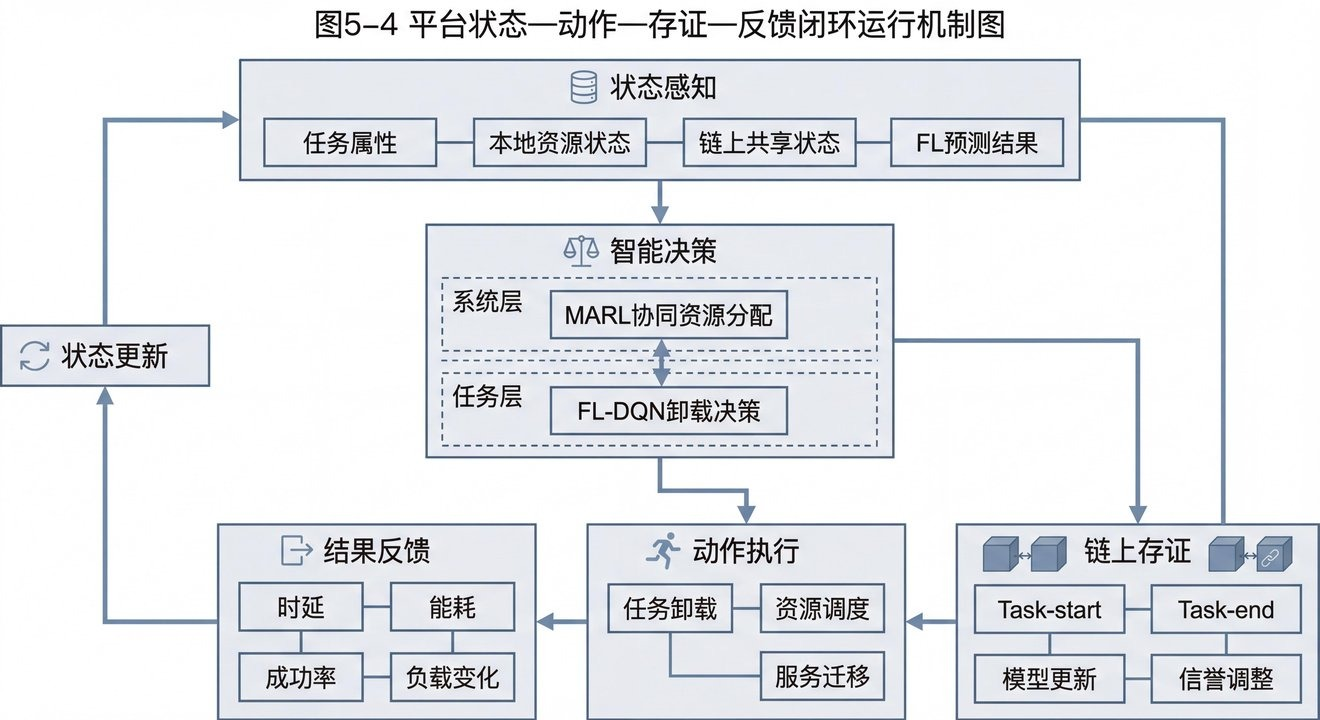
\includegraphics[width=0.92\textwidth]{figures/5-4.jpeg}
  \caption{平台状态—动作—存证—反馈闭环运行机制图}
  \label{fig:closed-loop}
\end{figure}

首先，平台在时刻\(t\)形成联合状态
\begin{equation}
  S(t)=\{S_p(t),O_{\mathrm{loc}}(t),G_{\mathrm{chain}}(t)\},
  \label{eq:joint_state}
\end{equation}
其中，\(S_p(t)\)表示式\eqref{eq:platform_state}定义的平台状态，\(O_{\mathrm{loc}}(t)\)表示节点本地观测集合，\(G_{\mathrm{chain}}(t)\)表示链上公共摘要集合。

其次，系统层基于较长时间尺度输出资源协同动作，任务层基于较短时间尺度输出卸载动作，平台联合动作表示为
\begin{equation}
  A(t)=\{a_{\mathrm{sys}}(t),a_{\mathrm{task}}(t)\}.
  \label{eq:joint_action}
\end{equation}
其中，\(a_{\mathrm{sys}}(t)\)通过式\eqref{eq:sys_to_task_constraint}转化为任务层约束，\(a_{\mathrm{task}}(t)\)通过式\eqref{eq:task_policy_platform}生成实际执行动作。

再次，动作执行过程中产生的关键事件被平台记录为链上事件集合
\begin{equation}
  E(t)=\{e_{\mathrm{submit}}(t),e_{\mathrm{accept}}(t),e_{\mathrm{start}}(t),e_{\mathrm{end}}(t),e_{\mathrm{model}}(t),e_{\mathrm{audit}}(t)\}.
  \label{eq:event_set}
\end{equation}
其中，任务提交、接纳、开始和结束事件构成任务生命周期链，模型事件对应联邦模型或策略模型的版本调用，审计事件用于记录异常证据和合约判定结果。

最后，任务执行结果被封装为反馈向量
\begin{equation}
  F(t)=\{L(t),E_c(t),Q(t),U(t),Z(t)\},
  \label{eq:feedback_vector}
\end{equation}
其中，\(L(t)\)表示时延反馈，\(E_c(t)\)表示能耗反馈，\(Q(t)\)表示任务完成质量，\(U(t)\)表示资源占用变化，\(Z(t)\)表示异常标记。平台状态更新为
\begin{equation}
  S_p(t+1)=\Phi\big(S_p(t),A(t),E(t),F(t),\Omega_{\mathrm{contract}}\big),
  \label{eq:closed_loop_update}
\end{equation}
其中，\(\Phi(\cdot)\)表示跨层闭环更新函数。式\eqref{eq:closed_loop_update}体现了本章平台的核心作用：系统层策略生成约束，任务层策略执行动作，区块链记录事件，执行结果更新状态，更新后的状态再反向影响下一轮系统层和任务层决策。

\section{平台运行流程与工程可行性分析}
\label{sec:platform_evaluation}

\subsection{平台运行流程}

以灾害应急遥感图像处理任务为例，平台运行过程可分为初始化、任务触发、模型校验、约束决策、执行存证、反馈回流和模型更新七个阶段。

初始化阶段，卫星节点同步最新主链区块头、子链状态摘要和模型版本目录，完成节点身份认证、权限确认和本地状态初始化。系统层模块根据链上负载摘要、链路统计和信誉状态，周期性输出资源协同策略，并将候选节点优先级和资源边界写入平台。

任务触发阶段，当某一卫星终端接收到高密度遥感图像识别任务后，首先提取任务计算量、输入数据大小、截止期和任务优先级，并采样本地CPU、缓存、队列长度和剩余能量等状态。同时，节点从链上公共信息板读取候选SEN的状态摘要和时间戳。

模型校验阶段，任务层模块向模型版本合约查询当前有效的并发开销预测模型版本，获得模型哈希、簇编号和聚合轮次。节点从链下模型库加载对应参数后重新计算哈希，若与链上记录一致，则进入预测与决策流程；否则触发模型异常审计或回退至上一稳定版本。

约束决策阶段，任务层模块读取系统层约束集合\(C_{\mathrm{limit}}(t)\)，过滤不可接纳任务或信誉低于阈值的候选节点，并调用联邦预测模型估计各候选动作的并发开销。随后DQN代理在受约束动作空间\(\mathcal{A}'_{\mathrm{task}}(t)\)中选择本地执行或目标节点卸载动作。

执行存证阶段，若目标节点满足平台约束并接纳任务，任务生命周期合约记录任务接纳和开始事件；若目标节点不满足约束或在可见窗口内不可达，则任务重新选择候选节点或回退至本地执行。任务执行完成后，平台记录完成状态、时延、能耗、结果摘要和异常标记。

反馈回流阶段，执行结果进入信誉更新合约和状态摘要合约。任务完成质量较高、时延和能耗满足约束的节点获得信誉提升；存在虚假上报、拒绝服务或异常失败的节点被扣减信誉，严重情况下触发异常隔离合约。更新后的资源状态、信誉状态和任务统计进一步进入系统层下一轮协同资源分配。

模型更新阶段，各节点基于本地历史执行日志构造并发开销监督样本，参与聚类联邦训练。聚合完成的新模型在链下保存完整参数，在链上登记版本号、参数哈希、簇编号和性能摘要。任务层节点在后续调用模型时依据链上登记信息完成版本校验。

\subsection{工程可行性评估设计}

为验证平台在天基动态环境下的可部署性，本章从确认时延、存储开销、异常治理和双层方法承载开销四个维度设计评估方案。仿真环境可结合STK生成星座轨道、可见窗口和链路连接关系，并利用NS-3构建网络层通信过程。在此基础上，平台层模拟主链—子链共识、跨链摘要提交、任务事件上链和链下对象存证流程。

表\ref{tab:platform_eval_param}给出了工程可行性评估的主要参数设置。具体数值可根据实际实验平台进行调整，本表主要用于说明第五章应关注的平台层指标，而非替代第3章和第4章的算法性能实验。

\begin{table}[htbp]
  \centering
  \caption{平台工程可行性评估参数设置}
  \label{tab:platform_eval_param}
  \begin{tabular}{p{4.0cm}p{8.5cm}}
    \toprule
    参数类别 & 设置说明 \\
    \midrule
    网络拓扑 & 由STK生成卫星轨道、星间链路可见性和星地链路窗口 \\
    通信仿真 & 由NS-3模拟链路带宽、传播时延、丢包和拥塞变化 \\
    共识节点规模 & 设置不同共识节点数量，用于评估确认时延随节点规模变化的趋势 \\
    交易类型 & 包括状态摘要交易、任务生命周期交易、模型版本交易和审计交易 \\
    存储方式 & 对比全量上链与“摘要上链+链下存储”两种方案 \\
    异常类型 & 包括虚假状态上报、延迟反馈、拒绝任务和异常模型更新 \\
    评价指标 & 平均确认时延、95分位确认时延、链上存储增长量、异常隔离时间、任务成功率恢复趋势 \\
    \bottomrule
  \end{tabular}
\end{table}

\subsection{确认时延与共识开销分析}

平台采用许可制联盟链结构，避免采用工作量证明等高消耗机制。对于天基协同计算场景，权威证明、拜占庭容错类轻量共识或基于信誉委托的共识机制均可作为候选方案。平台确认时延可近似分解为交易传播时延、验证时延、共识投票时延和区块广播时延：
\begin{equation}
  T_{\mathrm{confirm}}=T_{\mathrm{prop}}+T_{\mathrm{verify}}+T_{\mathrm{cons}}+T_{\mathrm{broadcast}}.
  \label{eq:confirm_delay}
\end{equation}

其中，\(T_{\mathrm{prop}}\)和\(T_{\mathrm{broadcast}}\)受星间/星地链路可见性和传播时延影响；\(T_{\mathrm{verify}}\)受交易复杂度和签名验证开销影响；\(T_{\mathrm{cons}}\)受共识节点规模和共识轮数影响。平台设计中将快时标任务事件优先写入子链，将全局治理和跨链锚定写入主链，有助于降低单条链上的交易拥塞，并使任务层决策无需等待所有全局信息实时确认。

从评估角度看，应重点绘制不同共识节点规模、不同交易到达率下的平均确认时延和95分位确认时延。如果确认时延远小于系统层资源协同周期，并且任务层实时决策主要依赖本地观测与最近链上摘要，则平台开销不会破坏第4章在线决策的实时性。需要强调的是，链上状态在本平台中提供的是可信但非实时的公共摘要，任务层DQN并不等待链上完成所有瞬时状态确认后再决策，而是结合本地观测和并发开销预测进行动作选择。

\subsection{存储增长与链上/链下协同分析}

若将任务输入、模型参数和详细执行日志全部上链，账本规模将随任务数量快速增长，并对卫星节点存储与同步造成较大压力。本章采用摘要上链和实体链下存储方式后，链上存储增长主要由任务事件摘要、状态摘要、模型版本摘要和审计索引构成。设时间窗内任务数量为\(N_T\)，模型更新次数为\(N_M\)，审计事件数量为\(N_A\)，则链上新增存储量可近似表示为
\begin{equation}
  S_{\mathrm{on}}=N_T s_{\mathrm{task}}+N_M s_{\mathrm{model}}+N_A s_{\mathrm{audit}}+N_S s_{\mathrm{state}},
  \label{eq:onchain_storage}
\end{equation}
其中，\(s_{\mathrm{task}}\)、\(s_{\mathrm{model}}\)、\(s_{\mathrm{audit}}\)和\(s_{\mathrm{state}}\)分别表示单条任务事件、模型版本、审计事件和状态摘要的链上记录大小，\(N_S\)表示状态摘要记录数量。

若采用全量上链方式，新增存储量可表示为
\begin{equation}
  S_{\mathrm{full}}=\sum_{j=1}^{N_D}|D_j|+N_T s_{\mathrm{task}}+N_M |M_j|+N_A s_{\mathrm{audit}},
  \label{eq:full_storage}
\end{equation}
其中，\(|D_j|\)表示链下数据对象大小，\(|M_j|\)表示完整模型参数大小。通常\(|D_j|\)和\(|M_j|\)远大于摘要大小，因此\(S_{\mathrm{on}}\ll S_{\mathrm{full}}\)。这说明链上/链下协同机制能够显著降低账本增长速度，使平台更适合资源受限的天基网络环境。

\subsection{异常节点隔离效果分析}

异常节点可能通过虚假上报资源状态、延迟反馈任务结果、拒绝执行已接纳任务或提交异常模型更新等方式破坏平台运行。平台通过任务生命周期合约、信誉更新合约和异常隔离合约形成闭环治理。评估时可设置一定比例的异常节点，观察其信誉值变化、被限权时间和系统任务成功率恢复趋势。

设异常节点集合为\(\mathcal{V}_{\mathrm{abn}}\)，平台的异常隔离目标不是立即删除所有异常节点，而是在证据充分的前提下降低其对任务调度和模型聚合的影响。可以采用如下指标衡量异常治理效果：
\begin{equation}
  \eta_{\mathrm{iso}}=\frac{|\mathcal{V}_{\mathrm{abn}}^{\mathrm{limited}}|}{|\mathcal{V}_{\mathrm{abn}}|},
  \label{eq:isolation_ratio}
\end{equation}
其中，\(\mathcal{V}_{\mathrm{abn}}^{\mathrm{limited}}\)表示被平台降权、限权或隔离的异常节点集合。若在异常注入后，节点信誉值能够随违规次数下降，异常节点逐步被移出候选卸载集合或降低联邦聚合权重，同时系统任务成功率逐步恢复，则说明平台治理机制对前文双层智能方法具有实际保护作用。

\subsection{对前文双层智能方法的承载作用}

平台工程分析的目的不在于重新证明第3章和第4章算法性能，而在于说明二者如何在同一个可信环境中协同运行。表\ref{tab:platform_support}总结了平台对前文方法的支撑作用。

\begin{table}[htbp]
  \centering
  \caption{平台对前文双层智能方法的承载作用}
  \label{tab:platform_support}
  \begin{tabular}{p{3.0cm}p{5.0cm}p{5.0cm}}
    \toprule
    支撑对象 & 平台提供的机制 & 对应作用 \\
    \midrule
    第3章系统层MARL & 公共状态摘要、信誉合约、策略审计、主链治理 & 支撑可信共享、信誉激励和长期协同资源分配 \\
    第4章联邦预测 & 模型版本合约、链下模型库、哈希校验、异常更新筛除 & 支撑模型版本可信维护和聚合结果追溯 \\
    第4章DQN卸载 & 候选节点摘要、系统层约束、任务生命周期合约 & 支撑实时决策输入、动作存证和结果回流 \\
    跨层闭环 & 约束传递接口、反馈回流接口、信誉更新与状态更新 & 支撑系统层与任务层之间的协同演化 \\
    工程部署 & 主链—子链结构、链上/链下存储、访问控制、审计查询 & 支撑轻量化、可扩展和可审计运行 \\
    \bottomrule
  \end{tabular}
\end{table}

由表\ref{tab:platform_support}可见，第5章并不是对第3章区块链公共信息板或第4章联盟链控制平面的简单重复，而是将二者扩展为统一的平台运行机制。第3章提供系统层全局协同能力，第4章提供任务层实时卸载能力，本章则通过分层联盟链、智能合约和链上/链下协同机制，使二者能够在同一平台中完成状态传递、规则约束、行为存证和反馈回流。

\section{本章小结}
\label{sec:platform_summary}

本章围绕前文双层智能方法如何在分布式天基环境中统一运行的问题，提出了一种面向天基协同计算的分层联盟链平台架构。与第3章侧重系统层协同资源分配算法、第4章侧重任务层并发感知卸载算法不同，本章重点从平台层解决状态共享、约束传递、模型治理、任务存证、信誉更新和执行反馈之间的统一承载问题。

首先，本章明确了平台设计需求和章节边界，指出第5章的核心任务不是重复说明区块链能够提供可信共享，而是将系统层全局协同结果转化为任务层可执行约束，并将任务层执行反馈回流为系统层状态更新和长期治理依据。其次，本章构建了基础设施与网络环境层、区块链平台核心层、双层智能决策层和应用与管理层构成的总体架构，并给出了平台状态模型和状态更新函数。再次，本章设计了主链—子链—链下设备层协同的分层联盟链机制，给出了字段化的主链和子链区块结构，并通过链上摘要与链下实体对象分离存储降低账本增长压力。随后，本章从节点准入、状态摘要、任务生命周期、模型版本、信誉更新和异常隔离六个方面设计智能合约治理机制，使任务执行、模型调用和异常处理具备自动执行与可审计能力。最后，本章重点给出了第3章系统层方法和第4章任务层方法的平台映射关系，建立了“状态—动作—存证—反馈”的跨层闭环，并从确认时延、存储增长、异常隔离和方法承载关系等角度分析了平台工程可行性。

通过上述设计，本章将第2章系统模型、第3章系统层协同优化方法与第4章任务层实时卸载方法统一映射到一个可运行、可验证、可审计的平台环境中，形成了从系统建模、算法设计到平台承载的完整研究链条。该平台为天基协同计算中的可信状态同步、跨层智能协同、联邦模型治理和执行结果回流提供了统一支撑，也为后续面向真实星座网络的工程部署和系统扩展奠定了基础。
